\documentclass[a4paper]{article}
\usepackage[utf8]{inputenc}
\usepackage[T1]{fontenc}
\usepackage[swedish,english]{babel} % english default language
\usepackage[binary-units]{siunitx}
\usepackage{graphicx}
\usepackage{booktabs}
\usepackage[style=alphabetic]{biblatex}
\addbibresource{literature.bib}
\usepackage{cleveref}

\author{Daniel Bosk}
\title{Test document}
\date{\today}

\begin{document}
\maketitle

\begin{abstract}
  This is the abstract, a short summary of the document.
  The document contains some examples.
\end{abstract}

\tableofcontents


\section{The first section}\label{sec:First}

We write some stuff in a paragraph.

Then we have another one.


\subsection{A subsection}\label{sub:Part}
Some more text.

We have the sum \(
  \sum_{i=1}^n i = \frac{n (n + 1)}{2}.
\) But we also have the sum \[
  \sum_{i=1}^n i = \frac{n (n + 1)}{2}.
\]
However, the following result is so great that we will reference it later.
\begin{equation}\label{TheGreatEquation}
  f(a) = \left\{
    \begin{array}{ll}
      y & \text{om } a=x \\
      x & \text{om } a=y
    \end{array}
  \right\} = f^{-1}(a).
\end{equation}


\section{References}\label{sec:Ref}

According to \textcite{Knuth1997tao}, there is no algorithm for solving the 
problem of coming up with the text to write\footnote{%
  Note that \citeauthor{Knuth1997tao} never said such a thing.
}.
But we are working hard on it.


\section{Figures and tables}\label{sec:FigTab}

Remember that great equation we had?
You know \cref{TheGreatEquation}.

You can also have a look at \cref{fig:bild,tbl:probabilities}.
But you should have read \cref{sec:First} first.

\begin{figure}
  \centering
  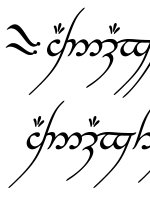
\includegraphics[width=0.2\linewidth]{tengwar.jpg}
  \caption{An example from J.~R.~R.~Tolkien's Tengwar.}
  \label{fig:bild}
\end{figure}

\begin{table}
  \centering
  \begin{tabular}{rcccccccccc}
    \toprule
    \(\alpha\) & a & b & c & d & e & f & g & h & i & j \\
    \(P_E(\alpha)\) & 8.2  & 1.5 & 2.8 & 4.3 & 12.7 & 2.2 & 2.0 & 6.1 & 7.0 & 0.2 \\
    \(P_S(\alpha)\) & 9.3  & 1.3 & 1.3 & 4.5 & 9.9 & 2.0 & 3.3 & 2.1 & 5.1 & 0.7 \\
    \bottomrule
  \end{tabular}
  \caption{Table of the probability function for letters of the English and 
  Swedish language, \(P_E\) and \(P_S\), respectively.
  Values are given as per cent with one decimal number precision.}
  \label{tbl:probabilities}
\end{table}

Many are confused by the units bits (\si{\bit}) and bytes (\si{\byte}).
One byte (\SI{1}{\byte}) consists of \SI{8}{\bit}.

To make matters worse, we use different prefixes.
We have that \SI{1}{\kilo\byte} is \SI{1000}{\byte}, but \SI{1}{\kibi\byte} is 
\SI{1024}{\byte} --- which is what computer scientists have traditionally used.


\printbibliography
\end{document}
